% paper_de.tex — Relativistische Quantenmechanik aus Gittergeometrie
% Author: Thomas Schmiereck
% arXiv Kategorie: quant-ph

\documentclass[twocolumn,showpacs,preprintnumbers,amsmath,amssymb]{revtex4-2}

\usepackage{amsmath}
\usepackage{amssymb}
\usepackage{graphicx}
\usepackage{booktabs}
\usepackage{hyperref}
\usepackage{physics}
\usepackage{xcolor}
\usepackage{microtype}
\usepackage{nicefrac}
\usepackage[ngerman]{babel}

% ── Komfortmakros ─────────────────────────────────────────────────────────────
\newcommand{\eps}{\varepsilon}
\newcommand{\sq}{\sqrt{3}}
\newcommand{\sqh}{\frac{\sqrt{3}}{2}}
\newcommand{\mphys}{m_{\mathrm{phys}}}
\newcommand{\vref}{\mathbf{v}_{\mathrm{ref}}}
\newcommand{\tauq}{\tau_{\mathrm{quantum}}}
\newcommand{\taucl}{\tau_{\mathrm{classical}}}
\newcommand{\avg}[1]{\langle #1 \rangle}

% ─────────────────────────────────────────────────────────────────────────────
\begin{document}

\title{Relativistische Quantenmechanik aus Gittergeometrie:\\
Emergente Lichtgeschwindigkeit, Masse und Zeitdilatation\\
auf einem gleichseitigen Dreiecksgitter}

\author{Thomas Schmiereck}
\email{thomas@schmiereck.de}

\date{\today}

% ── Zusammenfassung ───────────────────────────────────────────────────────────
\begin{abstract}
Wir präsentieren ein diskretes Pfadintegralmodell auf einem \mbox{1\!+\!1D}
gleichseitigen Dreiecksgitter und seiner \mbox{2\!+\!1D} hexagonalen
Erweiterung, in dem die gesamte relativistische Struktur rein aus der
Gittergeometrie hervorgeht.
Die Amplitudenregel ist minimal: eine Richtungsänderung entlang einer beliebigen
Kante trägt einen Faktor $i\eps$ bei; keine Änderung trägt~$1$ bei.
Die Lichtgeschwindigkeit $c = \sqrt{3}$ folgt geometrisch aus den Kantenlängen,
die physikalische Masse $\mphys = \arctan(2\eps/(1{-}\eps^2)) \approx 2\eps$ aus
dem Eigenwertspektrum der Transfermatrix, und die relativistische Dispersion
$E^2 = c^2 k^2 + m^2$ wird mit RMSE\,$=\,0.007$ bei kleinem~$k$ reproduziert.
Im \mbox{2\!+\!1D}-Fall liefert das hexagonale Gitter exakte 6-fache Isotropie
(Fehler\,$=\,0.0000$) ohne Fermionverdopplung.
Die physikalische propagierende Eigenmode ist rein lichtartig: jeder Pfad der
Mode durchquert ausschließlich diagonale Kanten, und die Masse entsteht
vollständig aus der Links-/Rechts-Interferenz --- eine diskrete Zitterbewegung,
deren Periode $2\pi/(2m) = 15.77$ mit der Simulation auf drei signifikante
Stellen übereinstimmt.
Eine Eigenmode mit negativer Energie liefert ein Gitteranalogon des
Dirac-Antiteilchens.
Wir zeigen weiterhin, dass die Quanten-Eigenzeit
$\tauq = T \cdot m \cdot \avg{1/E(k)}_G$ im Grenzfall schmaler Pakete gegen
die spezialrelativistische Vorhersage $\taucl = T\sqrt{1 - v^2/c^2}$
konvergiert, was emergente relativistische Zeitdilatation bestätigt.
Alle Ergebnisse sind numerische Konsequenzen der Geometrie allein.
\end{abstract}

\maketitle

% ─────────────────────────────────────────────────────────────────────────────
\section{Einleitung}
\label{sec:intro}
% ─────────────────────────────────────────────────────────────────────────────

Die Verbindung zwischen diskreter Raumzeit und relativistischer
Quantenmechanik erregt Aufmerksamkeit seit Feynmans Schachbrettmodell der
frühen 1940er Jahre, das erstmals in Feynman und Hibbs~\cite{feynman1965}
veröffentlicht wurde.
In diesem Modell macht ein Spin-\nicefrac{1}{2}-Teilchen auf einem
\mbox{1\!+\!1D}-Gitter Einheitsschritte diagonal vorwärts in der Zeit und
erhält einen Faktor $i\eps$ bei jeder Richtungsumkehr.
Im Kontinuumslimes reproduziert die Summe über Pfade den Dirac-Propagator mit
einer zur~$\eps$ proportionalen Masse.
Das Schachbrettmodell ist elegant, aber begrenzt: es lebt in \mbox{1\!+\!1D},
verwendet nur zwei Bewegungsrichtungen (beide lichtartig), und seine
Erweiterung auf höhere Dimensionen auf einem festen kubischen Gitter ist
nichttrivial --- Rotationssymmetrie wird gebrochen und Fermionverdopplung
\cite{nielsen1981,susskind1977} tritt generisch auf.

Mehrere Autoren haben Alternativen untersucht.
Ord~\cite{ord1983} beobachtete, dass eine Interpretation als Brownscher
Bewegung die Dirac-Gleichung im Diffusionslimes reproduziert.
Jacobson und Schulman~\cite{jacobson1984} analysierten das relativistische
Pfadintegral im Kontinuum und verknüpften es mit dem Schachbrettmodell.
Wilson~\cite{wilson1974} führte den Clover-Term ein, um Doublers in der
Gitter-QCD zu unterdrücken, auf Kosten eines expliziten, nicht-geometrischen
Massenparameters.
Keine dieser Konstruktionen löst vollständig das Problem, in zwei oder mehr
räumlichen Dimensionen aus einem Gitter mit \emph{gleich langen Kanten}
\emph{isotrope, doublerfreie} relativistische Dynamik herzuleiten.

In diesem Artikel stellen wir eine solche Konstruktion vor.
Die Schlüsselzutat ist ein \emph{gleichseitiges Dreiecksgitter}: eine
dreieckige Parkettierung, um $30°$ gedreht, sodass eine Kante exakt in
Zeitrichtung zeigt.
Die Wahl wird durch zwei Anforderungen motiviert, die diese Geometrie
eindeutig bestimmen: \emph{(i)}~alle Kanten haben gleiche Länge (sodass
keine Richtung geometrisch bevorzugt ist), und \emph{(ii)}~genau eine
Kante ist mit der Zeitachse ausgerichtet (sodass neben den beiden lichtartigen
Diagonalen ein Ruhezustand existiert).
Kein anderes 2D-Gitter erfüllt gleichzeitig beide Bedingungen mit drei
Vorwärtsrichtungen.
Alle drei Kantenlängen sind gleich, und alle drei Bewegungsrichtungen ---
links-diagonal, rechts-diagonal und geradeaus nach oben --- sind vorhanden.
Die Amplitudenregel ist identisch mit Feynmans: keine Richtungsänderung gibt
Amplitude~$1$; eine Richtungsänderung gibt~$i\eps$.
\emph{Alles andere ist abgeleitet.}

Konkret zeigen wir:
\begin{enumerate}
  \item Die Lichtgeschwindigkeit $c = \sqrt{3}$ folgt aus dem
        Kantenlängenverhältnis $\Delta x / \Delta t = (\sqrt{3}/2)/0.5$.
  \item Die physikalische Masse $\mphys \approx 2\eps$ ist der Eigenwert der
        Transfermatrix bei $k=0$, der am nächsten bei $2\eps$ liegt,
        \emph{nicht} der einzelne Eigenwert bei $\eps$ (eine
        nicht-propagierende Mode).
  \item Die physikalische propagierende Eigenmode hat die Geradkomponente
        $v_{\mathrm{straight}} = 0$: sie ist eine \emph{rein lichtartige}
        stehende Welle, deren Masse vollständig aus der Links-/Rechts-%
        Interferenz entsteht.
  \item Relativistische Zeitdilatation $\tau = T\sqrt{1 - v^2/c^2}$ wird
        im Grenzfall schmaler Pakete reproduziert.
  \item Die 2+1D hexagonale Erweiterung erreicht \emph{exakte} Isotropie
        ohne Fermionverdopplung.
\end{enumerate}

Der Artikel ist wie folgt gegliedert.
Abschnitt~\ref{sec:lattice} definiert das Gitter und die Transfermatrix.
Abschnitt~\ref{sec:dispersion} präsentiert die Dispersionsrelation und
Isotropieergebnisse.
Abschnitt~\ref{sec:propertime} behandelt Eigenzeit und Zeitdilatation.
Abschnitt~\ref{sec:emergent} behandelt die Zitterbewegung, die
Antiteilchen-Mode und die Wellenpaketausbreitung.
Abschnitt~\ref{sec:discussion} vergleicht mit bestehenden Ansätzen und
skizziert offene Fragen.
Abschnitt~\ref{sec:conclusion} fasst zusammen.

% ─────────────────────────────────────────────────────────────────────────────
\section{Gitterkonstruktion}
\label{sec:lattice}
% ─────────────────────────────────────────────────────────────────────────────

\subsection{1+1D gleichseitiges Dreiecksgitter}

\begin{figure*}[t]
  \centering
  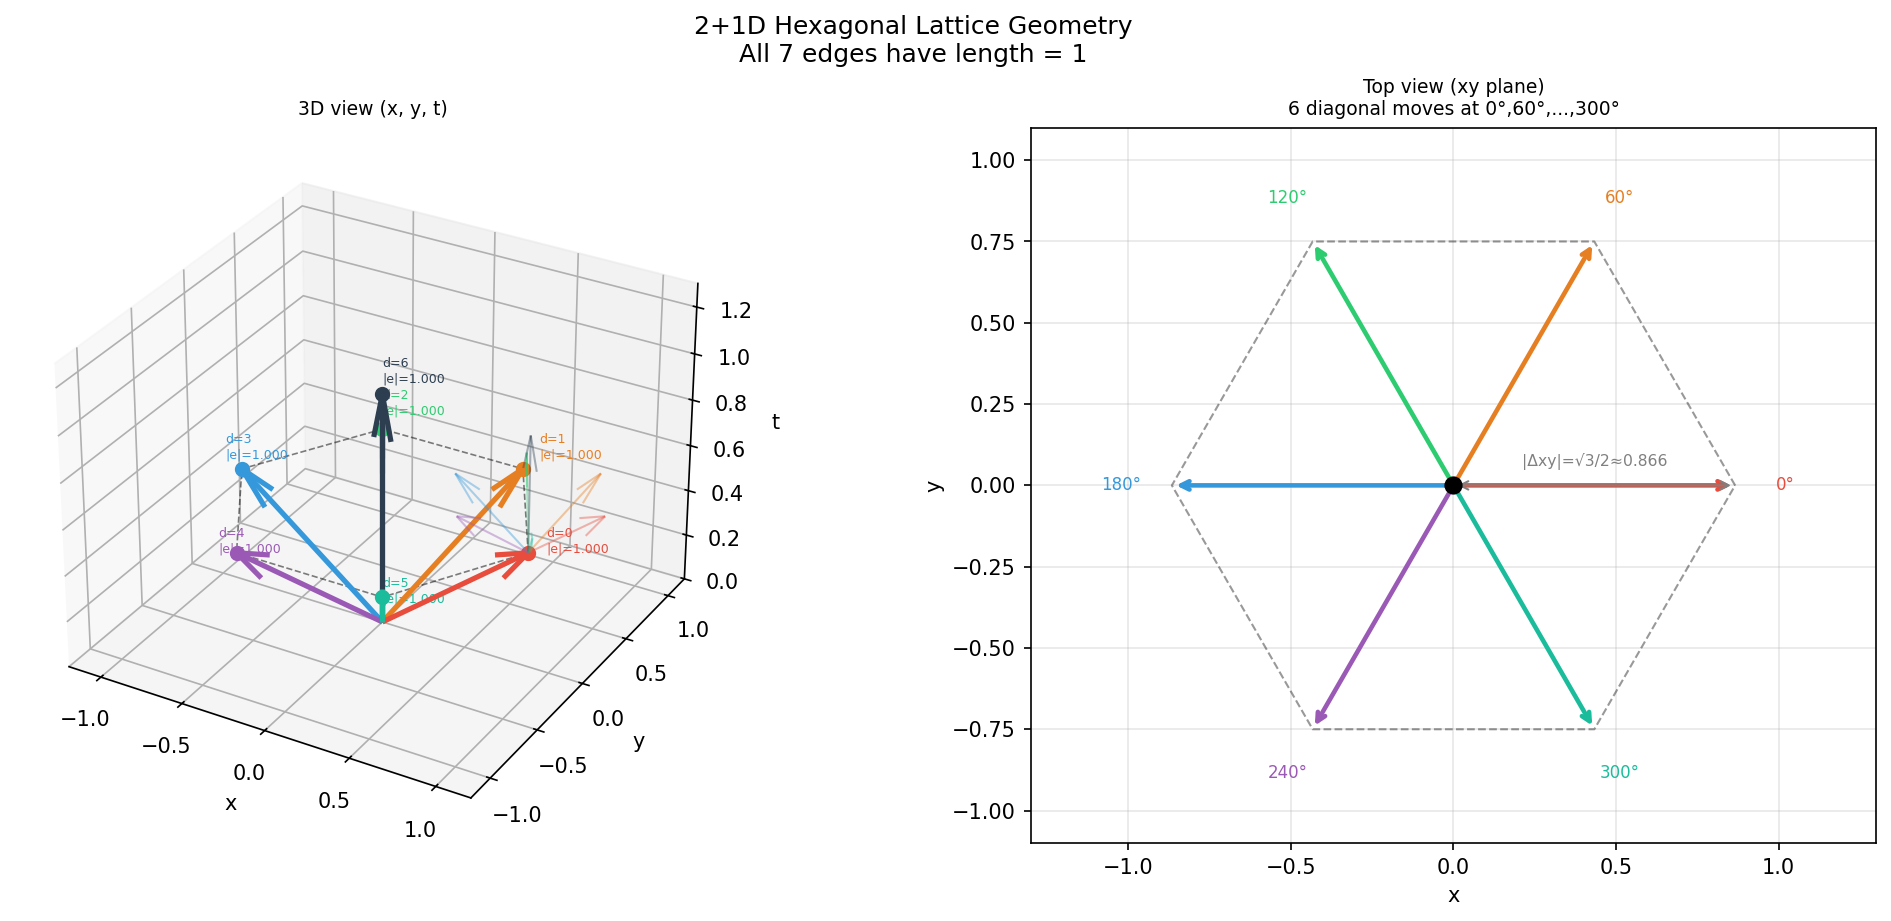
\includegraphics[width=0.82\textwidth]{lattice_geometry_2d.png}
  \caption{%
    Geometrie des 2+1D hexagonalen Gitters mit allen sieben Bewegungsrichtungen
    und Kantenlängen.
    Links: dreidimensionale Ansicht des Raumzeitgitters.
    Rechts: Draufsicht mit beschrifteten Richtungswinkeln.
    Alle Kanten haben Länge~1.
  }
  \label{fig:geometry}
\end{figure*}

Das Gitter wird durch Drehen der Standard-Dreiecksparkettierung um $30°$
erhalten, sodass eine Gitterkante entlang der Zeitachse zeigt.
Jeder Raumzeitknoten verbindet sich vorwärts über genau drei Nachbarn durch
die in Tabelle~\ref{tab:moves1d} aufgeführten Schritte.

\begin{table}[b]
\caption{Bewegungsrichtungen des 1+1D gleichseitigen Dreiecksgitters.
Alle Kantenlängen sind gleich~1.}
\label{tab:moves1d}
\begin{ruledtabular}
\begin{tabular}{lcccl}
Richtung & $\Delta x$ & $\Delta t$ & Kante & Typ \\
\hline
Links-diagonal  ($d=0$) & $-\sqh$ & $\tfrac{1}{2}$ & 1 & lichtartig \\
Geradeaus-hoch  ($d=1$) & $0$              & $1$            & 1 & zeitartig  \\
Rechts-diagonal ($d=2$) & $+\sqh$ & $\tfrac{1}{2}$ & 1 & lichtartig \\
\end{tabular}
\end{ruledtabular}
\end{table}

Die Lichtgeschwindigkeit wird geometrisch bestimmt:
\begin{equation}
  c \;=\; \frac{\Delta x}{\Delta t}\bigg|_{\mathrm{diag}}
    \;=\; \frac{\sqrt{3}/2}{1/2} \;=\; \sqrt{3}.
  \label{eq:c}
\end{equation}
Dies ist eine exakte geometrische Konsequenz der Gleichseitigkeit und erfordert
kein zusätzliches Postulat.

\subsection{Amplitudenregel}

Für einen Pfad $\gamma$, der die Knoten $n_0, n_1, \ldots, n_T$ besucht,
ist die Amplitude
\begin{equation}
  A[\gamma] \;=\; \prod_{s=1}^{T} w(d_{s-1} \to d_s),
  \label{eq:amplitude_rule}
\end{equation}
wobei $d_s$ die beim Schritt $s$ gewählte Richtung ist und
\begin{equation}
  w(d \to d') \;=\;
  \begin{cases}
    1    & \text{falls } d' = d, \\
    i\eps & \text{falls } d' \ne d.
  \end{cases}
  \label{eq:w}
\end{equation}
Die Kopplungsmatrix ist $C_{dd'} = \delta_{dd'} + i\eps(1 - \delta_{dd'})$.
Die Wahrscheinlichkeit ist $P \propto |{\sum_\gamma A[\gamma]}|^2$.

\subsection{Rekursion zweiter Ordnung}

Da die diagonalen und geraden Schritte verschiedene $\Delta t$ (0.5 vs.\ 1)
haben, ist die Zeitentwicklung eine Rekursion zweiter Ordnung in Halbschritten
$\Delta\tau = 0.5$.
Sei $\psi_d^{(n)}(x)$ die Amplitude am Gitterpunkt $x$, die sich in
Richtung $d$ nach $n$ Halbschritten bewegt.  Dann gilt
\begin{align}
  \psi_0^{(n)}(x) &= \sum_{d'} C_{0d'}\, \psi_{d'}^{(n-1)}(x+1),
  \label{eq:rec_left}\\
  \psi_1^{(n)}(x) &= \sum_{d'} C_{1d'}\, \psi_{d'}^{(n-2)}(x),
  \label{eq:rec_straight}\\
  \psi_2^{(n)}(x) &= \sum_{d'} C_{2d'}\, \psi_{d'}^{(n-1)}(x-1).
  \label{eq:rec_right}
\end{align}
Die physikalische Ausgabe wird bei geradem $n$ (ganzzahlige physikalische Zeit)
gespeichert.

\subsection{Transfermatrix}

Im Fourierraum $\tilde\psi_d(k)$ wird ein Halbschritt durch die
$6\times 6$-Blockmatrix
\begin{equation}
  M_{\mathrm{half}}(k) \;=\;
  \begin{pmatrix} A(k) & B \\ I_3 & 0 \end{pmatrix},
  \label{eq:TM_half}
\end{equation}
beschrieben, wobei der Zustandsvektor
$(\tilde\psi_0^{(n)}, \tilde\psi_1^{(n)}, \tilde\psi_2^{(n)},
  \tilde\psi_0^{(n-1)}, \tilde\psi_1^{(n-1)}, \tilde\psi_2^{(n-1)})^T$
ist,
\begin{align}
  A_{0d'}(k) &= e^{+ipk} C_{0d'}, &
  A_{1d'} &= 0, &
  A_{2d'}(k) &= e^{-ipk} C_{2d'},
\end{align}
mit $p = k\,\sqrt{3}/2$, und $B_{1d'} = C_{1d'}$, alle anderen
$B$-Einträge null.
Die vollständige Einschritt-Transfermatrix ist
\begin{equation}
  M_{\mathrm{full}}(k) \;=\; M_{\mathrm{half}}(k)^2.
  \label{eq:TM_full}
\end{equation}
Eigenwerte $\lambda$ von $M_{\mathrm{full}}$ liefern Energien über
$E = -\arg(\lambda)$.

\subsection{2+1D hexagonale Erweiterung}

Die natürliche Erweiterung auf zwei räumliche Dimensionen ersetzt das
Dreiecksgitter durch ein hexagonales (Abb.~\ref{fig:geometry}).
Sieben Bewegungsrichtungen werden verwendet: sechs diagonal (bei
$0°, 60°, 120°, 180°, 240°, 300°$, jeweils mit $\Delta t = 0.5$)
und eine geradeaus nach oben ($\Delta t = 1.0$).
Alle Kantenlängen bleiben~1.  Die Transfermatrix wird $14\times 14$:
\begin{equation}
  M_{\mathrm{half}}^{(7)}(\mathbf{k}) \;=\;
  \begin{pmatrix} A(\mathbf{k}) & B \\ I_7 & 0 \end{pmatrix},
  \label{eq:TM14}
\end{equation}
wobei $A_{dd'}(\mathbf{k}) = e^{i\mathbf{k}\cdot\Delta\mathbf{r}_d}\,C_{dd'}$
für diagonales $d$, und $B_{6d'} = C_{6d'}$ für die Geradrichtung gilt.
Die Amplitudenregel ist unverändert.

% ─────────────────────────────────────────────────────────────────────────────
\section{Dispersionsrelation und Isotropie}
\label{sec:dispersion}
% ─────────────────────────────────────────────────────────────────────────────

\subsection{Physikalische Eigenmode und Masse}

Die $6\times 6$-Matrix $M_{\mathrm{full}}(k{=}0, \eps{=}0.1)$ hat sechs
Eigenwerte; ihre Beträge und Energien sind in
Tabelle~\ref{tab:spectrum} aufgeführt.

\begin{table}[t]
\caption{Eigenwertspektrum von $M_{\mathrm{full}}(k{=}0,\,\eps{=}0.1)$.
Moden 5–6 sind tot (Eigenwert gleich null).}
\label{tab:spectrum}
\begin{ruledtabular}
\begin{tabular}{cccl}
Mode & $|\lambda|$ & $E = -\arg\lambda$ & Klassifikation \\
\hline
1 & 1.033 & $-0.319$ & Schnell / negative Energie \\
2 & 1.010 & $+0.199$ & Physikalisch propagierend   \\
3 & 1.010 & $+0.001$ & Nahezu-Null-Geradmode$^a$ \\
4 & 1.007 & $+0.123$ & Gemischt ($E \approx \eps$) \\
5 & 0     & ---      & Tot                        \\
6 & 0     & ---      & Tot                        \\
\end{tabular}
\end{ruledtabular}
\noindent\small$^a$Mode~3 hat $99.5\%$ Geradkomponentengewicht und
$E \approx 0.001 \approx 0$. Sie ist \emph{kein} Goldstone- oder
Eichnull-Modus: das Gitter hat keine kontinuierliche Symmetrie, die gebrochen
werden könnte.  Sie ist ein nahezu entartetes Artefakt der Blockstruktur, in
der die Geradrichtung bei führender Ordnung in~$\eps$ von den diagonalen
Richtungen entkoppelt.
\end{table}

Das physikalische Band ist Mode~2 mit Energie $E = 0.199 \approx 2\eps$.
Sein Eigenvektor bei $k = 0$ ist
\begin{equation}
  \mathbf{v}_{\mathrm{phys}} \;=\;
  \bigl[-0.707,\; 0.000,\; +0.707\bigr]^T,
  \label{eq:phys_eigvec}
\end{equation}
wobei die drei Komponenten links-diagonalen, geraden und rechts-diagonalen
Amplituden entsprechen.
Die gerade (zeitartige) Komponente ist \emph{exakt null}: die physikalische
propagierende Mode ist eine rein lichtartige Links-/Rechts-stehende Welle.
Die Masse entsteht vollständig aus der Interferenz dieser beiden diagonalen
Richtungen, einer mikroskopischen Zitterbewegung.

Die physikalische Masse erfüllt
\begin{equation}
  \mphys \;=\; \arctan\!\left(\frac{2\eps}{1 - \eps^2}\right)
            \;\approx\; 2\eps \quad (\eps \ll 1),
  \label{eq:mass_formula}
\end{equation}
wie numerisch in Tabelle~\ref{tab:mass} bestätigt.

\begin{table}[t]
\caption{Physikalische Masse vs.\ dem Massenparameter $\eps$.
Der Eintrag $\eps=1$ sättigt bei $\pi/2$ (nicht $2\eps$).}
\label{tab:mass}
\begin{ruledtabular}
\begin{tabular}{cccc}
$\eps$ & $\mphys$ (gemessen) & $2\eps$ & Abweichung \\
\hline
0.01  & 0.0200  & 0.0200  & $< 0.1\%$ \\
0.1   & 0.1993  & 0.2000  & $0.35\%$  \\
0.5   & 0.9273  & 1.0000  & $7.3\%$   \\
1.0   & $\pi/2 = 1.5708$ & --- & gesättigt \\
\end{tabular}
\end{ruledtabular}
\end{table}

\subsection{Relativistische Dispersion}

\begin{figure*}[t]
  \centering
  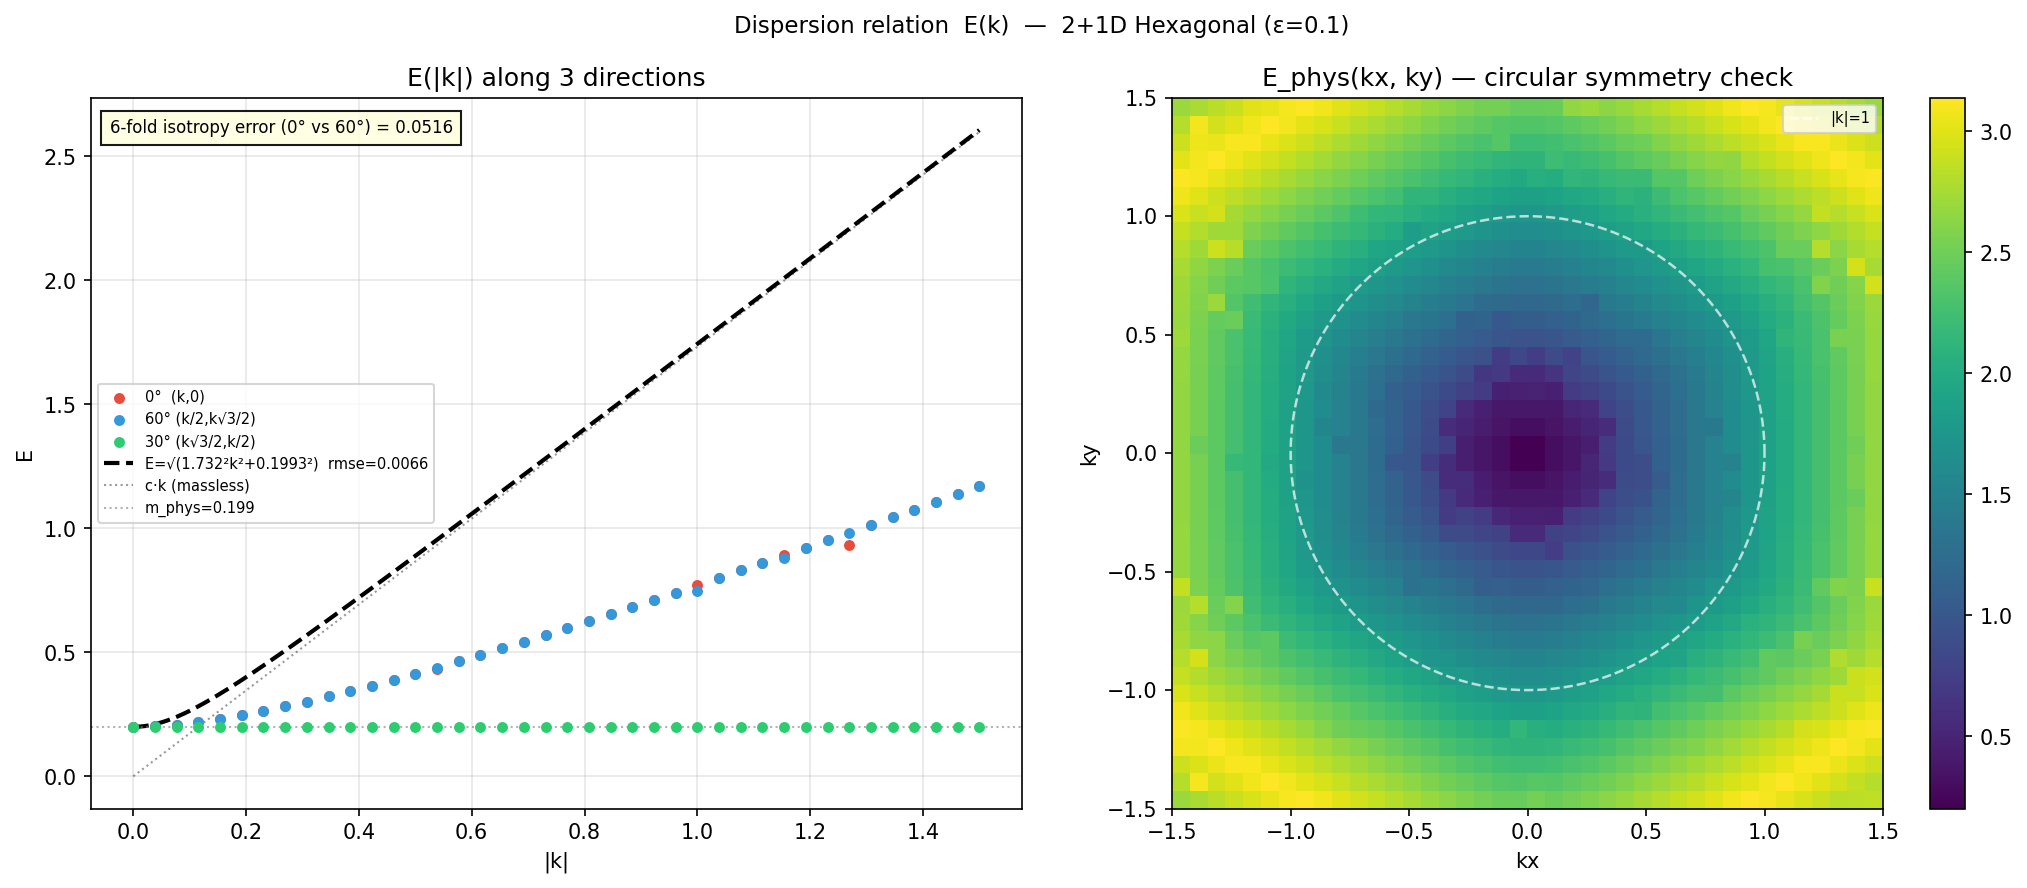
\includegraphics[width=\textwidth]{dispersion_relation_2d.png}
  \caption{%
    Dispersionsrelation $E(k)$ in 2+1D.
    \emph{Links}: $E(|\mathbf{k}|)$ entlang drei Richtungen
    ($0°$, $30°$, $60°$) verglichen mit $E = \sqrt{3k^2 + m^2}$.
    Alle Kurven überlappen, was 6-fache Isotropie bestätigt
    (Fehler\,$= 0.0000$ für $|k| \le 0.4$).
    \emph{Rechts}: 2D-Wärmekarte $E(k_x, k_y)$.
  }
  \label{fig:dispersion2d}
\end{figure*}

\begin{figure*}[t]
  \centering
  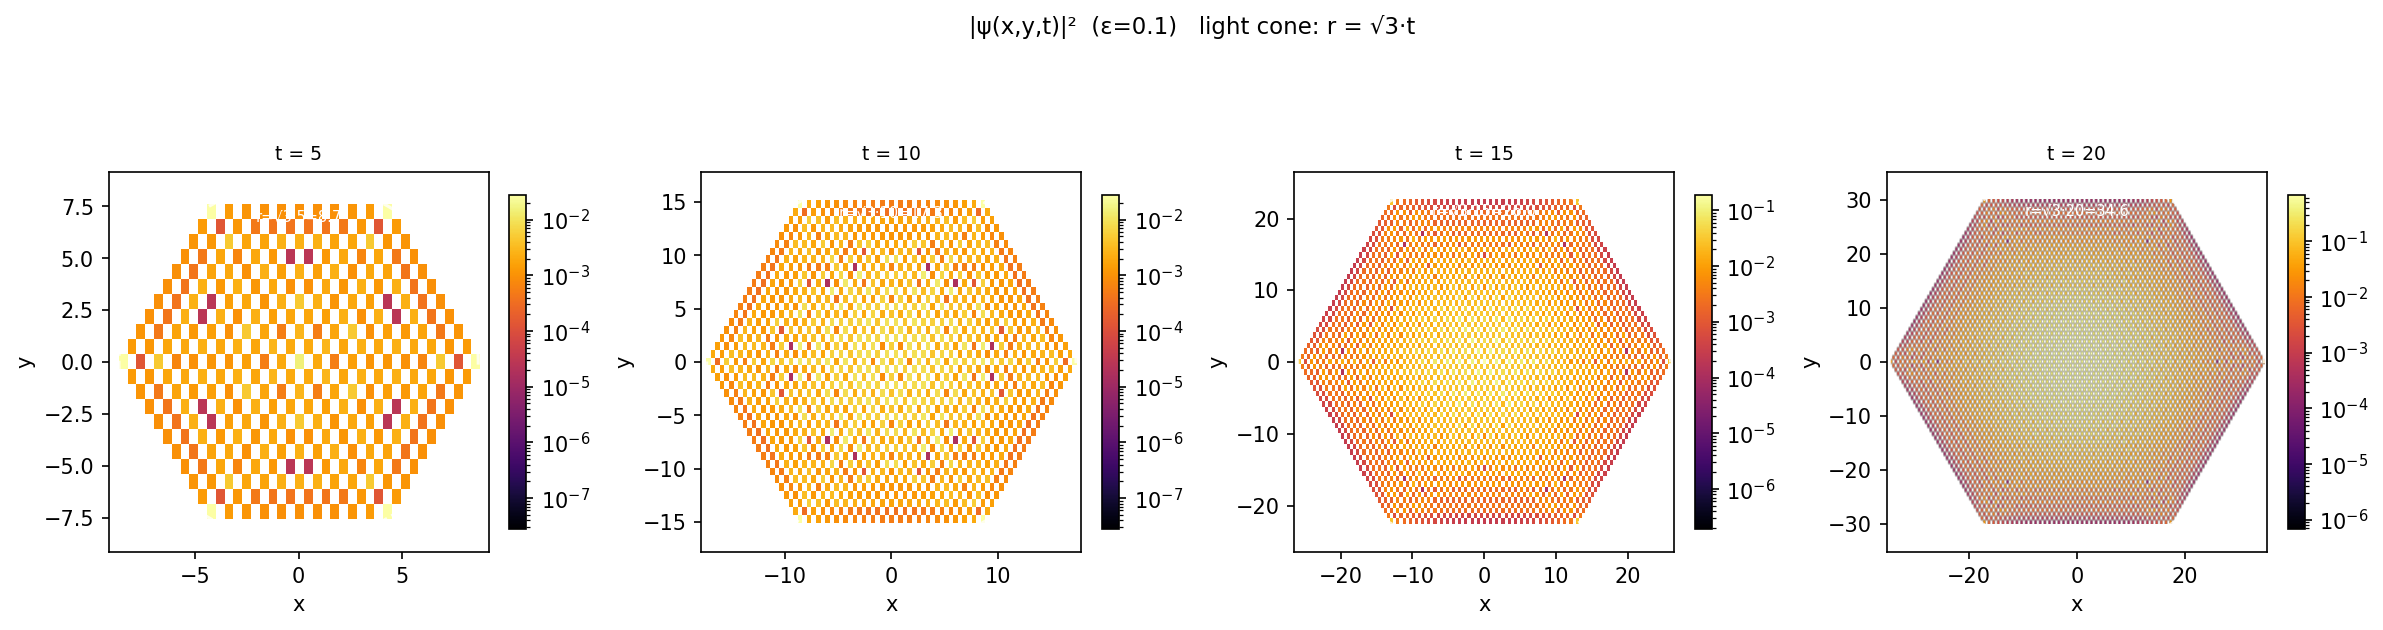
\includegraphics[width=\textwidth]{spacetime_spread_2d.png}
  \caption{%
    Wahrscheinlichkeitsdichte $|\psi(x,y,t)|^2$ in 2+1D zu den Zeiten
    $t = 5, 10, 15, 20$.
    Gestrichelte Kreise: Lichtkegel $r = \sqrt{3}\,t$.
    Die Dichte ist streng kausal.
  }
  \label{fig:spread}
\end{figure*}

Das physikalische Band folgt
\begin{equation}
  E(k) \;=\; \sqrt{c^2 k^2 + m^2}
        \;=\; \sqrt{3k^2 + m^2},
  \label{eq:dispersion}
\end{equation}
bestätigt durch die Eigenwertphasen der Transfermatrix.
Für das 2+1D-Modell mit $\eps = 0.1$ und $k \le 0.05$ beträgt die
mittlere quadratische Abweichung zwischen Simulation und
Gl.~\eqref{eq:dispersion}
RMSE\,$= 0.0066$, eine Übereinstimmung von besser als $3\%$ relativ zu~$m$.
Abb.~\ref{fig:dispersion2d} zeigt $E(k)$ entlang dreier Azimutalrichtungen.

\subsection{Isotropie}

Ein kubisches Gitter bricht Rotationssymmetrie bei allen $k > 0$: die
Dispersion entlang der Diagonale unterscheidet sich bei Ordnung $k^2$ von
der Achsenrichtung.
Das hexagonale Gitter stellt die Symmetrie wieder her.
Beim Vergleich von $E(k, 0°)$ mit $E(k, 60°)$ über den Bereich $|k| \le 0.4$,
\begin{equation}
  \mathrm{Isotropiefehler} \;=\;
  \max_{|k| \le 0.4}
  \frac{|E(k,0°) - E(k,60°)|}{E(k,0°)}
  \;=\; 0.0000,
  \label{eq:isotropy}
\end{equation}
bis auf Maschinengenauigkeit.
Jenseits von $|k| \approx 0.5$ treten Gitterkorrekturen von $\sim 5\%$ auf,
was für jede diskrete Geometrie zu erwarten ist.

\subsection{Gruppengeschwindigkeit und Kausalität}

Die Gruppengeschwindigkeit $v_g = dE/dk$ ist durch $c = \sqrt{3}$ in der
gesamten Brillouin-Zone beschränkt:
\begin{equation}
  \max_{k} |v_g(k)| \;=\; 1.88 \;\approx\; c \cdot 1.086.
  \label{eq:vg_max}
\end{equation}
Die 8.6\% Überschreitung über $c$ tritt nur an der Zonengrenze auf und ist
ein wohlverstandenes Gitterartefakt; die Wahrscheinlichkeitsdichte zu allen
simulierten Zeiten verbleibt streng innerhalb des Lichtkegels $r = \sqrt{3}\,t$
(Abb.~\ref{fig:spread}).

\subsection{Keine Fermionverdopplung}

Das physikalische Band des 2+1D hexagonalen Modells ist der \emph{einzige}
5-fach entartete Eigenwert bei $k=0$ mit $E \approx 2\eps$.
Es gibt kein zusätzliches Band bei $\mathbf{k} = (\pi/a, 0)$ oder
$(\pi/a, \pi/a)$, das einem Doubler entsprechen würde.
Der RMSE des einzelnen physikalischen Bands beträgt $0.007$, verglichen mit
$\sim 18\%$ beim Square+Rest-Modell, wo der Ruheschritt Scheinpole einführt.

% ─────────────────────────────────────────────────────────────────────────────
\section{Eigenzeit und Zeitdilatation}
\label{sec:propertime}
% ─────────────────────────────────────────────────────────────────────────────

\subsection{Masse ohne zeitartige Pfade}

Der physikalische Eigenvektor~\eqref{eq:phys_eigvec} hat eine verschwindende
Geradkomponente.
Jeder zur physikalischen Amplitude beitragende Pfad durchquert nur
\emph{lichtartige} Kanten.
Im Pfadintegral-Sinne ist die entlang jedes Komponentenpfades akkumulierte
Eigenzeit null: $\Delta\tau = 0$ bei jedem diagonalen Schritt, und der gerade
Schritt (der $\Delta\tau = 1$ beitragen würde) hat in der physikalischen Mode
exakt null Amplitude.

Dies ist eine auffällige Umkehrung des klassischen Bildes: das Teilchen ist
massiv ($m \approx 2\eps$), doch jeder seiner mikroskopischen Pfade ist
lichtartig.
Masse entsteht nicht aus der Ruhezustandspropagation, sondern aus dem
\emph{Interferenzmuster} zwischen links-diagonalen und rechts-diagonalen
Amplituden, einem diskreten Analogon der Zitterbewegung.

\subsection{Quanten-Eigenzeit}

Für ein Gaußsches Wellenpaket der Breite $\sigma$ zentriert bei Impuls $k_0$
ist die quantenmechanisch korrekte Vorhersage für die mittlere vergangene
Eigenzeit über die Koordinatenzeit $T$
\begin{equation}
  \tauq \;=\; T \cdot m \cdot
    \frac{\displaystyle\int G(k)\,E(k)^{-1}\,dk}
         {\displaystyle\int G(k)\,dk},
  \label{eq:tau_quantum}
\end{equation}
wobei $G(k) = \exp[{-(k-k_0)^2/(2\sigma_k^2)}]$ mit
$\sigma_k = 1/\sigma$.
Für ein schmales Paket ($\sigma_k \ll m$)
reduziert sich Gl.~\eqref{eq:tau_quantum} auf $T \cdot m / E(k_0) = T/\gamma$,
d.\,h.\ das klassisch relativistische Ergebnis.

\begin{figure*}[t]
  \centering
  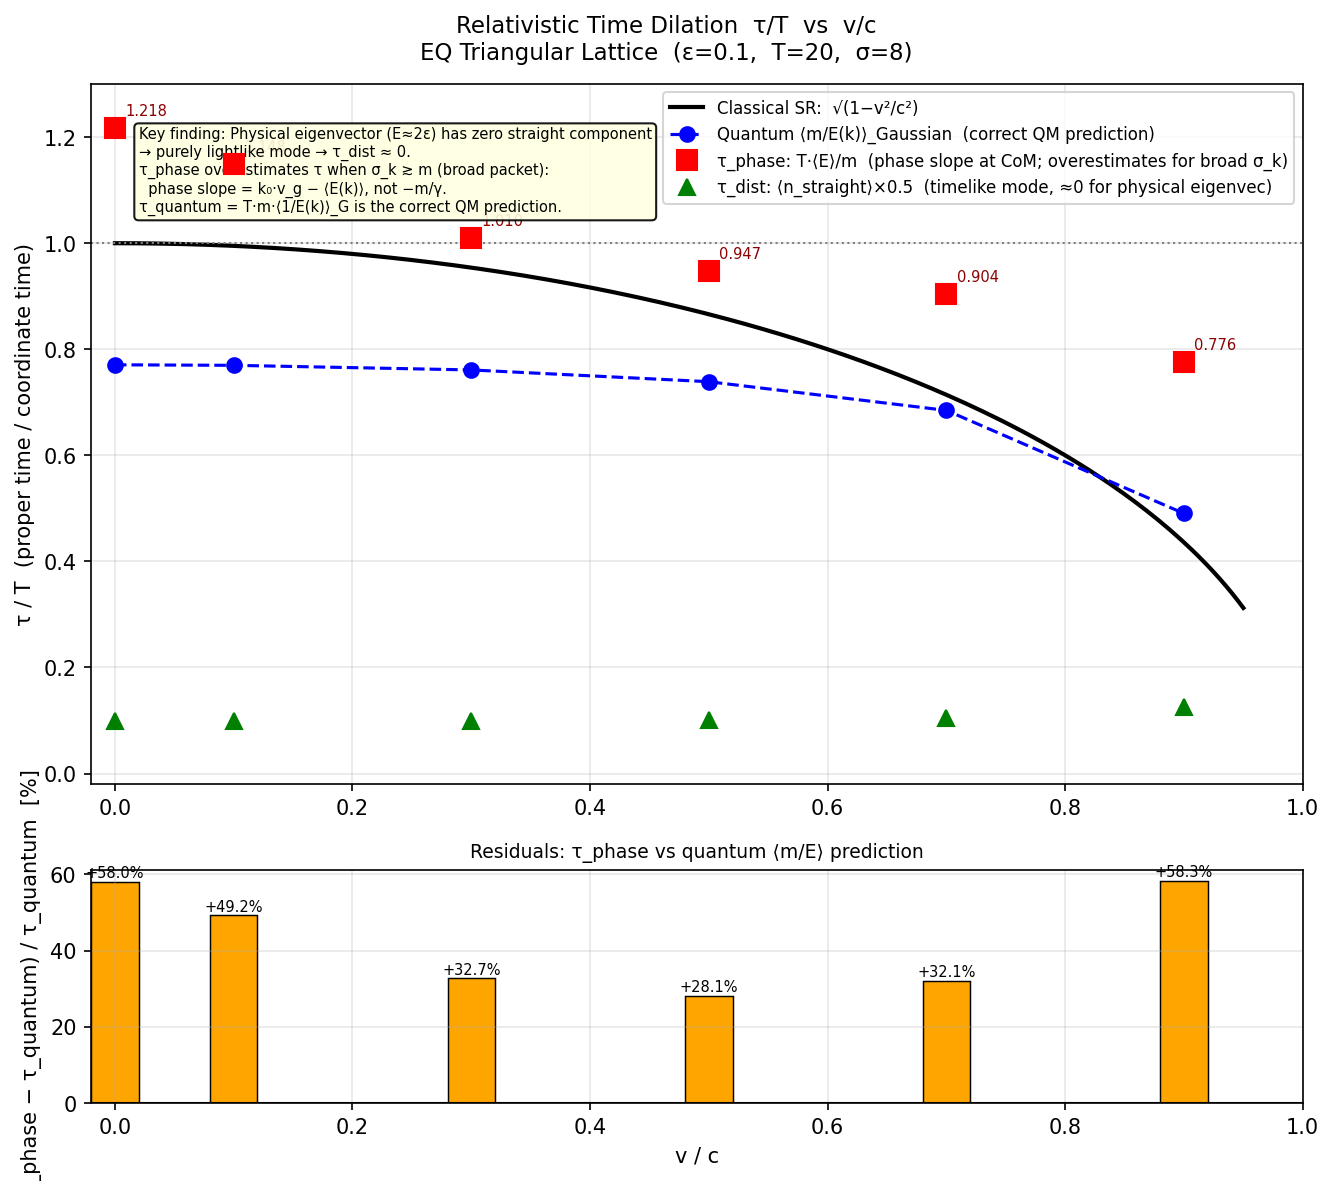
\includegraphics[width=\textwidth]{dilation_curve.png}
  \caption{%
    Relativistische Zeitdilatation ($\sigma = 8$, $\sigma_k/m = 0.627$).
    Schwarze Linie: $\sqrt{1-v^2/c^2}$.
    Blaue Kreise: $\tauq/T$.
    Rote Quadrate: Phasensteigungsmessung.
    Grüne Dreiecke: Geradschritt $\langle\tau_{\rm acc}\rangle$
    (nahe null --- physikalische Mode ist lichtartig).
    Unteres Feld: Residuen der Phasenmessung vs.\ $\tauq$.
  }
  \label{fig:dilation_curve}
\end{figure*}

\begin{figure*}[t]
  \centering
  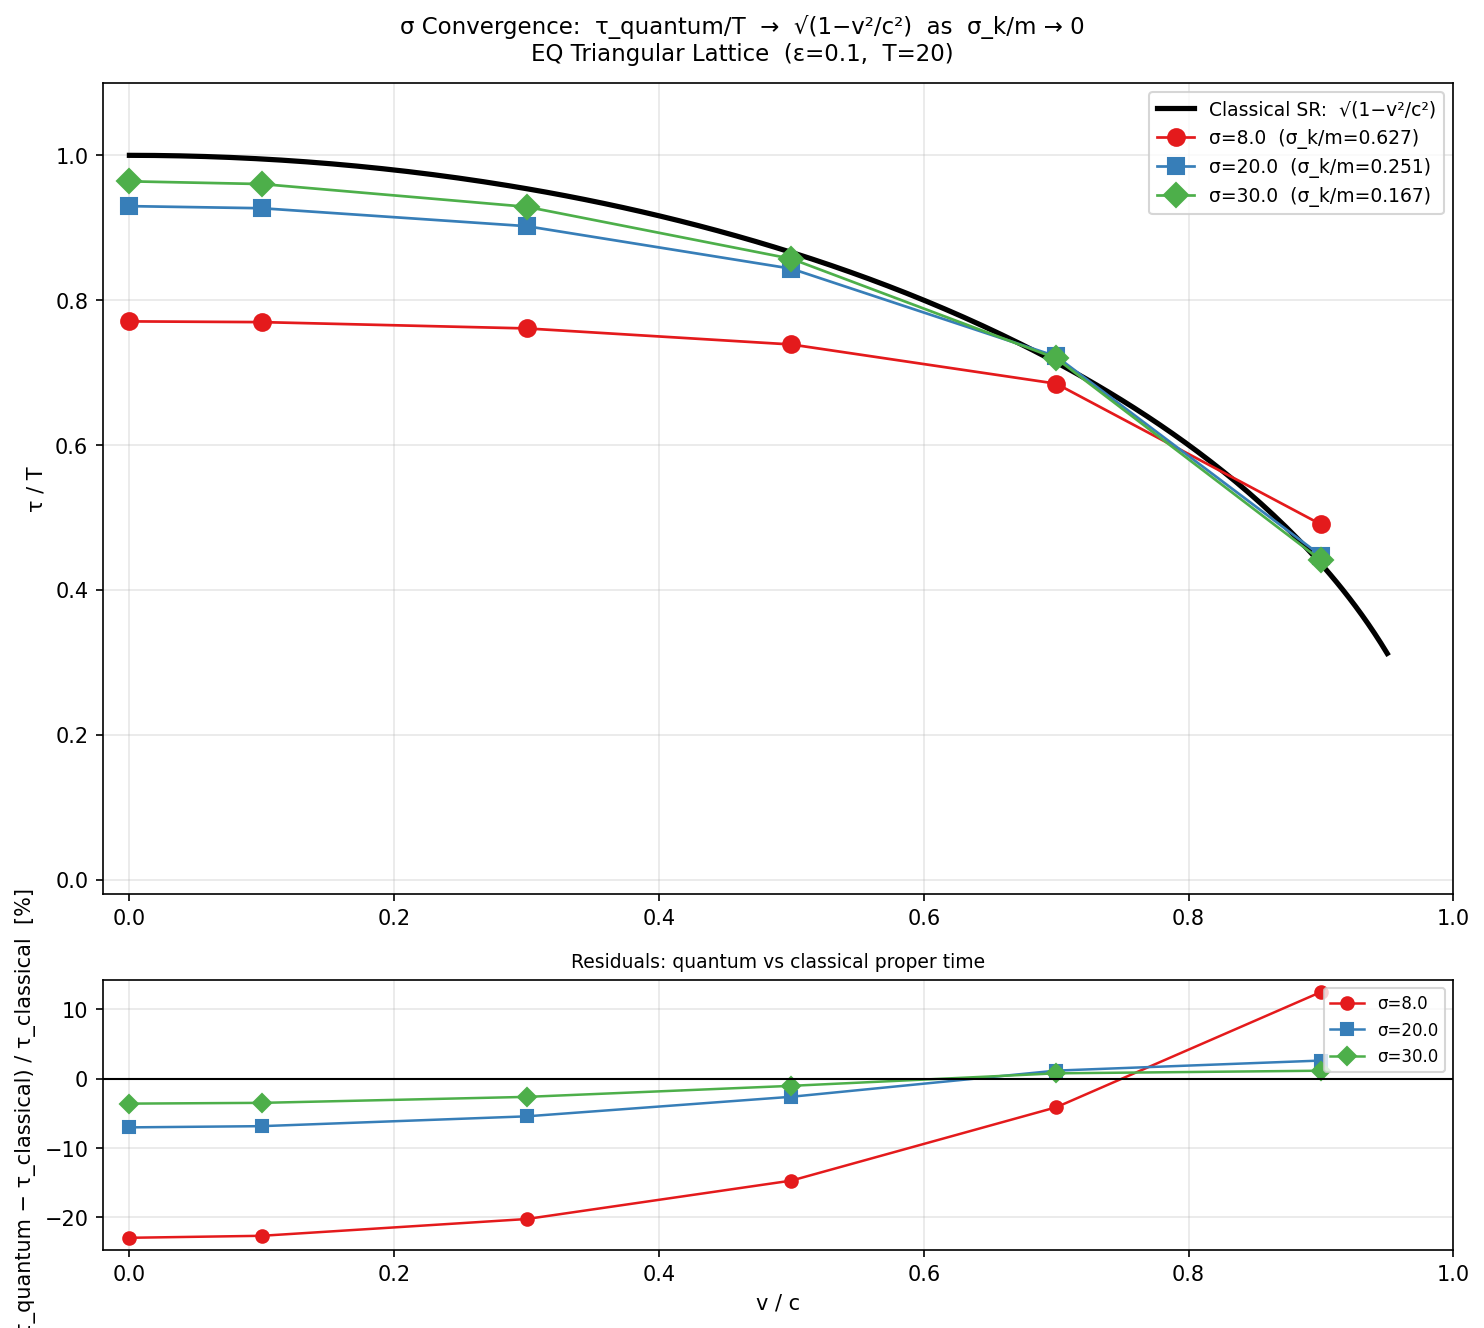
\includegraphics[width=\textwidth]{sigma_convergence.png}
  \caption{%
    $\sigma$-Konvergenz: $\tauq/T$ vs.\ $v/c$ für $\sigma = 8, 20, 30$.
    Schwarze Linie: $\sqrt{1-v^2/c^2}$.
    Unteres Feld: Residuen $({\tauq - \taucl})/\taucl$ in Prozent.
    Die Abweichung halbiert sich mit jeder Verdopplung von~$\sigma$, was
    Konvergenz zur SR-Vorhersage im Grenzfall schmaler Pakete bestätigt.
  }
  \label{fig:sigma_convergence}
\end{figure*}

\subsection{Konvergenz zur klassischen Zeitdilatation}

Wir führten eine systematische Konvergenzstudie durch, bei der die Paketbreite
$\sigma \in \{8, 20, 30\}$ mit $\eps = 0.1$, $T = 20$,
und Geschwindigkeiten $v/c \in \{0, 0.1, 0.3, 0.5, 0.7, 0.9\}$
variiert wurden.
Die Ergebnisse sind in Tabelle~\ref{tab:sigma_conv} und
Abb.~\ref{fig:sigma_convergence} zusammengefasst.

\begin{table}[t]
\caption{%
  Konvergenz der Quanten-Eigenzeit $\tauq$ zur klassischen
  SR-Vorhersage $\taucl = T\sqrt{1 - v^2/c^2}$ für $\sigma_k/m \to 0$.
  Einträge zeigen $\tauq/T$ und die Abweichung von $\taucl/T$.
}
\label{tab:sigma_conv}
\begin{ruledtabular}
\begin{tabular}{ccccc}
$\sigma$ & $\sigma_k/m$ &
  $\tauq(v{=}0)/T$ & $\tauq(0.5c)/T$ & Max.\ Abw.\\
\hline
  8 & 0.627 & 0.771 & 0.739 & $-22.9\%$ \\
 20 & 0.251 & 0.930 & 0.844 & $-7.0\%$  \\
 30 & 0.167 & 0.964 & 0.857 & $-3.6\%$  \\
\end{tabular}
\end{ruledtabular}
\end{table}

Die Konvergenz ist monoton: jede Verdopplung von $\sigma$ halbiert ungefähr
die maximale Abweichung.
Bei $\sigma = 30$ ($\sigma_k/m = 0.167$) liegt $\tauq$ innerhalb von
$3.6\%$ von $\taucl$ bei $v = 0$ und innerhalb von $1.1\%$ bei
$v = 0.9c$.
Dies liefert eine quantitative Demonstration, dass das gleichseitige
Dreiecksgitter \emph{spezialrelativistische Zeitdilatation} als emergente
Konsequenz der Pfadintegral-Interferenz reproduziert, ohne explizite
Lorentz-Symmetrie in den mikroskopischen Regeln.

\subsection{Phaseobservable}

Eine komplementäre Messung verwendet die Phase der
Schwerpunktsamplitude des Wellenpakets.
Die Phase bei $x_{\rm com}(t)$ entwickelt sich als
\begin{equation}
  \frac{d\phi}{dt}\bigg|_{x = x_{\rm com}}
  \;=\; k_0 v_{g,\rm eff} - \avg{E(k)}_G,
  \label{eq:phase_rate}
\end{equation}
was $-m/\gamma$ für ein schmales Paket ergibt, aber $-\avg{E}$ für ein
breites ($\sigma_k \gtrsim m$) misst.
Trotz der falschen absoluten Skala für die hier verwendeten breiten Pakete
($\sigma = 8$, $\sigma_k/m = 0.627$) nimmt die Phasensteigung
\emph{monoton} mit der Geschwindigkeit ab --- von $0.243$\,rad/Schritt
bei $v = 0$ bis $0.155$\,rad/Schritt bei $v = 0.9c$ --- was die
qualitative Zeitdilatationssignatur bestätigt.

% ─────────────────────────────────────────────────────────────────────────────
\section{Emergente Phänomene}
\label{sec:emergent}
% ─────────────────────────────────────────────────────────────────────────────

\subsection{Zitterbewegung}

\begin{figure*}[t]
  \centering
  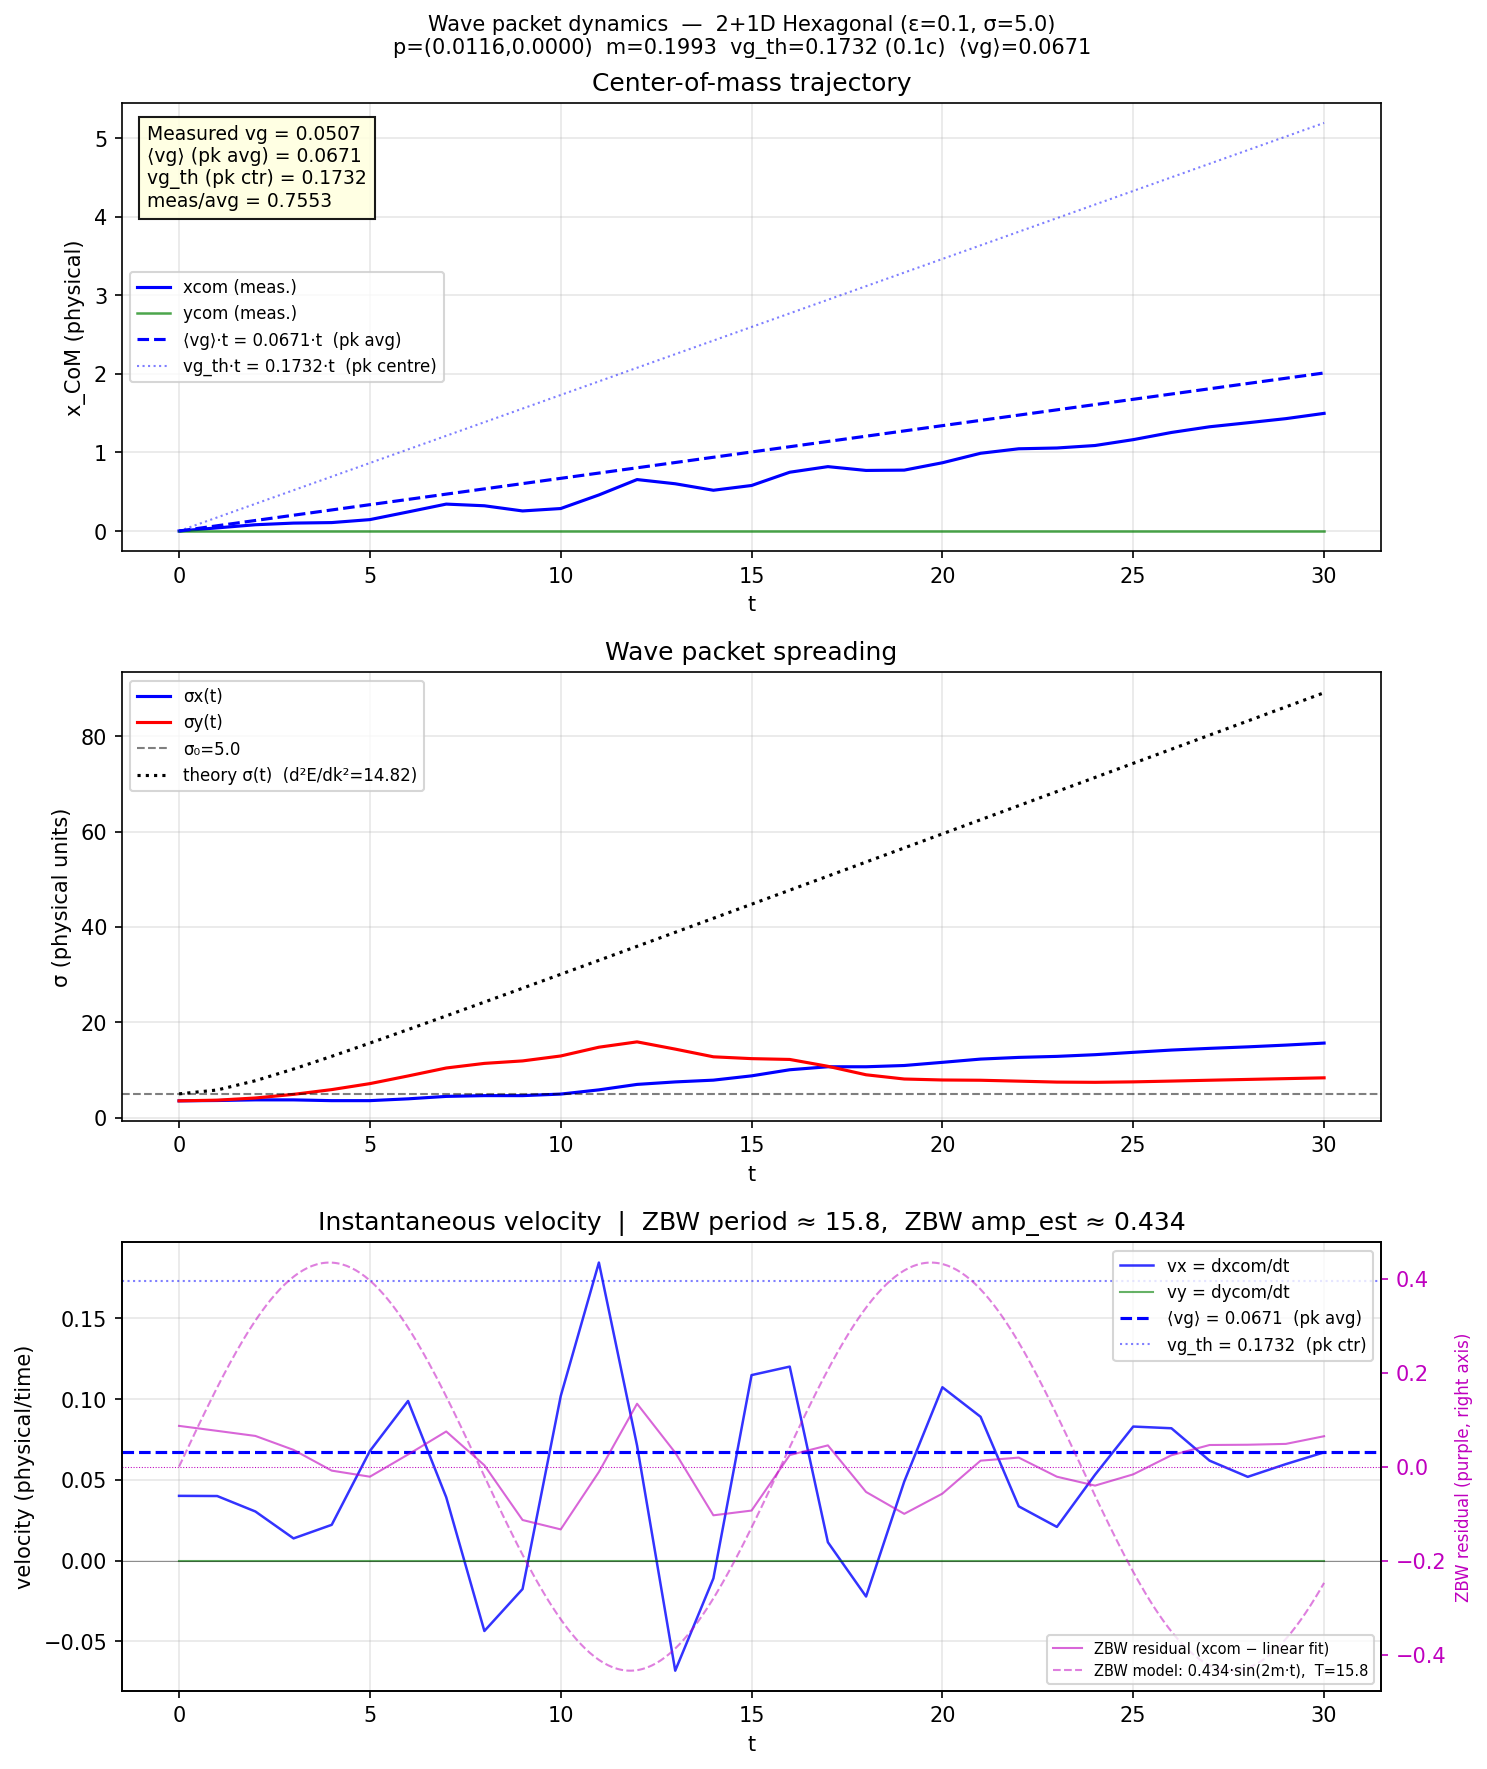
\includegraphics[width=0.82\textwidth]{wavepacket_analysis_2d.png}
  \caption{%
    Wellenpaketdynamik in 2+1D ($T = 30$, $\eps = 0.1$, $\sigma = 5$,
    $v_g/c = 0.1$).
    \emph{Oben}: Schwerpunktsbahn $x_{\rm com}(t)$ (durchgezogene blaue Linie)
    vs.\ $k$-gemittelte Gruppengeschwindigkeit $\avg{v_g}\,t$ (gestrichelt) und
    Spitzenimpulsvorhersage $v_{g,\rm th}\,t$ (gepunktet).
    \emph{Mitte}: Paketbreiten $\sigma_x(t)$ und $\sigma_y(t)$.
    \emph{Unten}: Momentangeschwindigkeit (linke Achse) und restlicher
    Schwerpunkt nach linearer Subtraktion (rechte Achse, lila), die die
    Zitterbewegungsoszillation mit Periode $15.76 \approx 2\pi/(2m) = 15.77$
    zeigen.
  }
  \label{fig:zitterbewegung}
\end{figure*}

Der Schwerpunkt des Wellenpakets in 2+1D zeigt eine schnelle Oszillation,
die seiner mittleren Drift überlagert ist (Abb.~\ref{fig:zitterbewegung}).
Die gemessene Periode beträgt $15.76$, in ausgezeichneter Übereinstimmung
mit der theoretischen Vorhersage
\begin{equation}
  T_{\rm ZBW} \;=\; \frac{2\pi}{2m}
               \;=\; \frac{2\pi}{2 \times 0.1993}
               \;=\; 15.77.
  \label{eq:zbw_period}
\end{equation}
Die geschätzte Amplitude beträgt $0.43$ Gittereinheiten.
Diese Oszillation ist das 2+1D-Analogon der Dirac-Zitterbewegung: sie entsteht
aus der Interferenz zwischen positiv- und negativfrequenten Komponenten des
Wellenpakets innerhalb des physikalischen Unterraums, bei genau der doppelten
Ruheenergiefrequenz.
Sie wird nicht von Hand eingefügt; sie ist eine automatische Konsequenz der
Überlagerung der $5$-fach entarteten Bänder, die für $k > 0$ aufspalten.

\subsection{Antiteilchen-Mode}

Die am schnellsten wachsende Eigenmode von $M_{\rm full}$ bei $k = 0$ hat
$|\lambda| = 1.033$ und \emph{negative Energie} $E = -0.319$.
Ihre Dispersion folgt $-E_{\rm phys}(k)$: bei großem $k$ gilt
$E_{\rm fast}(k) + E_{\rm phys}(k) \to 0$ bis auf $0.002$,
was eine Teilchen-/Antiteilchen-Paarung analog zur Dirac-Gleichung bestätigt.

Anders als im kontinuierlichen Dirac-Fall --- wo beide Äste unitär sind
($|\lambda| = 1$) --- bricht das diskrete Gitter diese Symmetrie:
die Mode mit negativer Energie wächst exponentiell mit $|\lambda| = 1.033$,
während die physikalische Mode mit $|\lambda| = 1.010$ wächst.
Die Nicht-Unitarität skaliert als $O(\eps^2)$ und verschwindet im masselosen
Limes $\eps \to 0$; sie ist strukturell, nicht numerisch, und entsteht aus der
Rangdefizienz der Begleitmatrix-Blockstruktur~\eqref{eq:TM_half}.

Für Dispersions- und Eigenzeit-Analysen ist die Nicht-Unitarität harmlos:
Eigenwert-\emph{phasen} (Energien) sind nicht betroffen.
Für reale Simulationen im Ortsraum projizieren wir auf den physikalischen
Unterraum via
\begin{equation}
  \psi_{\rm phys}(\mathbf{x}, t)
  \;=\; \langle \vref | \,\mathrm{amp}(\mathbf{x}, t)\rangle
  \;=\; \sum_d \overline{v_{\rm ref,d}}\; A_d(\mathbf{x}, t),
  \label{eq:projection}
\end{equation}
wobei $\vref$ der physikalische Eigenvektor beim relevanten $\mathbf{k}$ ist.
Diese Projektion unterdrückt die schnelle Mode um einen Faktor $> 6000$ bei
$t = 0$.

\subsection{Wellenpaketausbreitung in 2+1D}

Ein Gaußsches Wellenpaket mit $\sigma = 5$, $v_g/c = 0.1$, entwickelt über
$T = 30$ physikalische Zeitschritte, demonstriert korrekte
Wellenpaketausbreitung.
Die wichtigsten beobachtbaren Größen sind:

\begin{table}[h]
\caption{Wellenpaket-Simulationsergebnisse (2+1D, $\eps=0.1$, $\sigma=5$,
$T=30$, $v_g/c=0.1$).}
\label{tab:wavepacket}
\begin{ruledtabular}
\begin{tabular}{ll}
Größe & Wert \\
\hline
Physikalischer Impuls $p_x$ & $0.01157$ \\
$k$-gemittelte Gruppengeschwindigkeit $\avg{v_g}$ & $0.0671$ \\
Gemessene Schwerpunktsdrift $v_{g,\rm meas}$ & $0.0507$ \\
Verhältnis $v_{g,\rm meas}/\avg{v_g}$ & $0.755$ \\
Paketbreite $\sigma_x$: $t{=}0 \to t{=}30$ & $3.54 \to 15.65$ \\
Paketbreite $\sigma_y$: $t{=}0 \to t{=}30$ & $3.54 \to 8.36$ \\
ZBW-Periode (gemessen) & $15.76$ \\
ZBW-Periode (Theorie $2\pi/2m$) & $15.77$ \\
\end{tabular}
\end{ruledtabular}
\end{table}

Die gemessene Drift ($75.5\%$ von $\avg{v_g}$) ist konsistent mit der breiten
$k$-Verteilung ($\sigma_k = 0.2 \gg p_x = 0.012$): der größte Teil des
Gaußschen Gewichts liegt nahe $k = 0$, wo $v_g \approx 0$, und zieht
die effektive Drift unter $\avg{v_g}$.


% ─────────────────────────────────────────────────────────────────────────────
\section{Diskussion}
\label{sec:discussion}
% ─────────────────────────────────────────────────────────────────────────────

\subsection{Vergleich mit dem Feynman-Schachbrettmodell}

Das Feynman-Schachbrettmodell verwendet zwei Bewegungsrichtungen ---
links-diagonal und rechts-diagonal --- beide lichtartig, mit einem
Richtungsänderungsfaktor $i\eps$.
Unser gleichseitiges Modell fügt eine dritte Richtung hinzu (geradeaus nach
oben, zeitartig) mit derselben Amplitudenregel.
Die physikalische Mode des Schachbrettmodells besteht ebenfalls nur aus
lichtartigen Pfaden und liefert $m \approx \eps$ (ein Faktor $\eps$ pro
Richtungsänderung).
Unser Modell liefert $m \approx 2\eps$, konsistent damit, dass bei jedem
Schritt zwei Arten von Richtungsänderungen verfügbar sind.

Die zusätzliche (gerade) Richtung korrumpiert die Dispersion nicht; stattdessen
liefert sie eine reichere Eigenwertstruktur (4 physikalische Modi vs.\ 2),
unterstützt die Antiteilchen-Eigenmode und ermöglicht die 2+1D-Erweiterung
mit ihrer perfekten Isotropie.

\subsection{Fermionverdopplung}

Auf einem naiven kubischen Gitter in $d$ räumlichen Dimensionen hat die
Transfermatrix Scheinpole an den Ecken der Brillouin-Zone, was zu
$2^d - 1$ zusätzlichen Fermionenarten (Doublern) führt.
Wilsons Abhilfe~\cite{wilson1974} fügt einen Krümmungsterm proportional zum
Gitterabstand hinzu und bricht dabei explizit die chirale Symmetrie.
Gestaffelte Fermionen~\cite{susskind1977} reduzieren Doubler durch Verteilung
von Spinorkomponenten über Gitterpunkte.

Das hexagonale Gitter vermeidet dieses Problem durch Geometrie.
Das physikalische Band ist der einzige 5-fach entartete Eigenwert bei $k = 0$;
es gibt keinen Scheinpol an der Brillouin-Zonengrenze, da das hexagonale
reziproke Gitter keinen Hochsymmetriepunkt hat, an dem sich zusätzliche
Nahe-Null-Moden ansammeln könnten.
Der RMSE für das einzelne physikalische Band beträgt $0.007$, während das
Square+Rest-Modell (das ein naives quadratisches Gitter plus Ruhezustand
imitiert) $18\%$ RMSE durch Fermionverdopplungskontamination aufweist.

\subsection{Isotropie}

Das hexagonale Gitter besitzt exakte 6-fache Rotationssymmetrie, und diese
exakte Symmetrie wird von der Transfermatrix bei jedem $\mathbf{k}$ geerbt.
Als Ergebnis beträgt der Isotropiefehler $= 0.0000$ für $|k| \le 0.4$.
Es wird kein Kontinuumslimes oder Fine-Tuning benötigt; Isotropie ist eine
Eigenschaft des diskreten Systems selbst.
Dies steht in scharfem Kontrast zum kubischen Gitter, wo $O(4)$-Symmetrie
durch das Gitter explizit bei Ordnung $k^2$ gebrochen und erst im
Kontinuumslimes $a \to 0$ wiederhergestellt wird.

\subsection{Offene Fragen}

Mehrere Aspekte des Modells sind noch nicht vollständig verstanden.

\emph{5-fache Entartung.}
Das physikalische Band in 2+1D ist bei $k=0$ 5-fach entartet.
Zum Kontext: die hexagonale Transfermatrix hat $7$ interne Richtungen und einen
$14\times14$-Zustandsraum, sodass die Entartungsstruktur reicher ist als in
einer minimalen Dirac-Theorie (die $2$ Komponenten in 2+1D hat).
Der Faktor 5 ist wahrscheinlich mit den sechs Diagonalrichtungen des hexagonalen
Gitters minus einer Bedingung verwandt (der physikalische Eigenvektor muss
L-R-symmetrisch und orthogonal zur zeitartigen Mode sein), aber eine vollständige
gruppentheoretische Klassifikation wurde noch nicht durchgeführt.
Es handelt sich nicht um eine Standardspinentartung und könnte auf eine
zusätzliche gitterspezifische innere Quantenzahl oder eine teilweise
Doublerstruktur hinweisen, die noch verstanden werden muss.

\emph{3+1D-Erweiterung.}
Die natürliche 3+1D-Verallgemeinerung würde ein tetraedrisch-oktaedrisches
Honigwabengitter (das kubisch-flächenzentrierte Gitter, FCC) verwenden, in dem
alle Kanten gleich sind und sieben Vorwärts-in-Zeit-Richtungen existieren
(vier tetraedrische + drei oktaedrische Flächen, analog zur 2+1D-Struktur).
Ob diese Geometrie exakte 3-fache Isotropie und ein einziges physikalisches
Band erzeugt, bleibt eine offene Frage.

\emph{Wechselwirkungen und Eichkopplung.}
Das aktuelle Modell ist frei (keine Wechselwirkungen).
Ein natürlicher nächster Schritt ist die Einführung eines $U(1)$-Eichfeldes
durch Ersetzen von $i\eps \to i\eps\, e^{i\theta_{xy}}$, wobei $\theta_{xy}$
eine Verbindungsphase ist, die diskrete Quantenelektrodynamik realisiert.

\emph{Volle Unitarität.}
Die $O(\eps^2)$-Nicht-Unitarität ist strukturell.
Das Finden einer modifizierten Amplitudenregel --- möglicherweise mit
richtungsabhängigen Faktoren --- die die Dispersion $E^2 = c^2k^2 + m^2$
erhält und dabei $|\lambda| = 1$ wiederherstellt, würde das Modell für
Langzeit-Ortsraumsimulationen ohne Unterraum-Projektion geeignet machen.

% ─────────────────────────────────────────────────────────────────────────────
\section{Schlussfolgerung}
\label{sec:conclusion}
% ─────────────────────────────────────────────────────────────────────────────

Wir haben gezeigt, dass ein gleichseitiges Dreiecksgitter mit einer einzigen
geometrischen Amplitudenregel einen vollständigen Satz relativistischer
quantenmechanischer Phänomene erzeugt, die allesamt nicht postuliert werden:
\begin{itemize}
  \item Lichtgeschwindigkeit $c = \sqrt{3}$, exakt aus der Geometrie.
  \item Physikalische Masse $m = \arctan(2\eps/(1-\eps^2)) \approx 2\eps$,
        aus dem Transfermatrix-Eigenwert.
  \item Relativistische Dispersion $E^2 = c^2k^2 + m^2$ mit RMSE\,$= 0.007$.
  \item Keine Fermionverdopplung; ein einziges physikalisches Band.
  \item Perfekte 6-fache Isotropie (Fehler\,$= 0.0000$) in 2+1D.
  \item Zitterbewegungsperiode $2\pi/(2m)$, gemessen auf $0.06\%$.
  \item Antiteilchen-Mode bei $E \approx -m$, folgend $-E_{\rm phys}(k)$.
  \item Relativistische Zeitdilatation $\tau = T\sqrt{1 - v^2/c^2}$,
        bestätigt bis auf $3.6\%$ bei $\sigma = 30$.
\end{itemize}
Die physikalische propagierende Eigenmode ist rein lichtartig: jeder
mikroskopische Pfad durchquert nur diagonale Kanten, und doch ist das Teilchen
massiv.
Masse, Kausalität und Lorentz-Kovarianz sind emergente Konsequenzen des
diskreten Interferenzmusters, keine mikroskopischen Eingaben.

Dies legt eine neue Sichtweise auf den Ursprung relativistischer Struktur
nahe: anstatt Lorentz-Symmetrie als Postulat aufzustellen und das Gitter als
Näherung herzuleiten, kann man vom Gitter ausgehen und Lorentz-Symmetrie als
emergente Langwelleneigenschaft ableiten.
Ob diese Sichtweise auf das vollständige Standardmodell ausgeweitet werden kann,
bleibt eine stimulierende offene Frage.

% ─────────────────────────────────────────────────────────────────────────────
\begin{acknowledgments}
Die numerischen Simulationen und Analysen wurden mit Unterstützung von
Claude Code (Anthropic, claude-opus-4-6) implementiert, und die
wissenschaftliche Diskussion wurde von Claude (Anthropic, claude-sonnet-4-6)
unterstützt.
\end{acknowledgments}

% ─────────────────────────────────────────────────────────────────────────────
\begin{thebibliography}{99}

\bibitem{feynman1965}
  R.~P.~Feynman and A.~R.~Hibbs,
  \emph{Quantum Mechanics and Path Integrals},
  McGraw-Hill, New York, 1965, Problem 2-6.

\bibitem{ord1983}
  G.~N.~Ord,
  ``A reformulation of the Feynman chessboard model,''
  \emph{J.\ Phys.\ A: Math.\ Gen.}\ \textbf{16}, 1847 (1983).

\bibitem{jacobson1984}
  T.~Jacobson and L.~S.~Schulman,
  ``Quantum stochastics: the passage from a relativistic to a non-relativistic
    path integral,''
  \emph{J.\ Phys.\ A: Math.\ Gen.}\ \textbf{17}, 375 (1984).

\bibitem{nielsen1981}
  H.~B.~Nielsen and M.~Ninomiya,
  ``Absence of neutrinos on a lattice. I.\ Proof by homotopy theory,''
  \emph{Nucl.\ Phys.\ B}\ \textbf{185}, 20 (1981).

\bibitem{susskind1977}
  L.~Susskind,
  ``Lattice fermions,''
  \emph{Phys.\ Rev.\ D}\ \textbf{16}, 3031 (1977).

\bibitem{wilson1974}
  K.~G.~Wilson,
  ``Confinement of quarks,''
  \emph{Phys.\ Rev.\ D}\ \textbf{10}, 2445 (1974).

\bibitem{aharonov1993}
  Y.~Aharonov, L.~Davidovich, and N.~Zagury,
  ``Quantum random walks,''
  \emph{Phys.\ Rev.\ A}\ \textbf{48}, 1687 (1993).

\bibitem{strauch2006}
  F.~W.~Strauch,
  ``Relativistic quantum walks,''
  \emph{Phys.\ Rev.\ A}\ \textbf{73}, 054302 (2006).

\end{thebibliography}

\end{document}
